\chapter{Introducción}
\label{ch:Introduccion}
\pagenumbering{arabic} 

En este proyecto se construirá material docente para la enseñanza de robótica utilizando diversas tecnologías. Para saber cual es el marco de desarrollo y dónde se engloban los conceptos utilizados vamos a introducir algunos términos que servirán como contexto y que permitirán entender mejor de dónde surge la necesidad de estos escenarios y la utilidad de los mismos.

\section{Robótica}
\label{sec:intr_robotica}

Según la Wikipedia\cite{wikipedia}, \textit{La robótica es la rama de la ingeniería mecatrónica, de la ingeniería eléctrica, de la ingeniería electrónica, de la ingeniería mecánica, de la ingeniería biomédica y de las ciencias de la computación que se ocupa del diseño, construcción, operación, disposición estructural, manufactura y aplicación de los robots.}

Otra definición menos técnica podría ser: La robótica es una ciencia o rama de la tecnología, que estudia el diseño y construcción de máquinas capaces de desempeñar tareas realizadas por el ser humano o que requieren del uso de inteligencia. Por tanto, estamos ante una ciencia que se encarga de diseñar máquinas que sean capaces de reemplazar al ser humano en algunas acciones. Es una disciplina con sus propios problemas, sus fundamentos y sus leyes, y podemos observar dos vertientes de la misma, la teórica y la práctica. En la parte teórica podemos agrupar todas las aportaciones de la informática, la inteligencia artificial y la automatización. En cuanto a la parte práctica observamos aportaciones relativas tanto a la construcción del robot como a la de su gestión, siendo por tanto destacadas las aportaciones de la mecánica, electrónica, programación, etc. Esto hace de la robótica una ciencia con un marcado carácter interdisciplinario.

\subsection{Historia de la robótica}
\label{subsec:intr_historiarobotica}

La historia de la robótica ha estado unida a la construcción de “artefactos”, que trataban de materializar el deseo humano de crear seres semejantes a nosotros que nos descargasen del trabajo. Desde los primeros pasos de la civilización el ser humano ha desarrollado ingenios tanto para facilitar sus labores como para imitar a la naturaleza, fascinando a sus congéneres. De los antiguos egipcios se conservan descripciones de más de 100 máquinas y autómatas, (incluyendo un artefacto con fuego, un órgano de viento, una máquina operada mediante una moneda, una máquina de vapor) en la obra \textit{Pneumática y Autómata} de Herón de Alejandría. Los griegos nos dejaron creaciones como un pájaro de madera, a vapor, que fue capaz de volar, y genios como Leonardo da Vinci el diseño de un \textit{Caballero mecánico}. 

En el año 1921 un escritor checo, Karel Capek, publica su obra \textit{“Los Robots Universales de Rossum”}, en la que aparece por primera vez la palabra “robot“ derivada de la palabra checa robota, que significa servidumbre o trabajo forzado. Unos años más tarde, en 1942, la revista americana \textit{Astounding Science Fiction} pública "Círculo Vicioso" (Runaround en inglés), una historia de ciencia ficción escrita por Isaac Asimov donde aparecen por primera vez las Tres leyes de la robótica. Estas leyes establecen lo siguiente:
\begin{quote}
\begin{enumerate}[1.ª]
	\item Un robot no hará daño a un ser humano o, por inacción, permitir que un ser humano sufra daño.
	\item Un robot debe hacer o realizar las órdenes dadas por los seres humanos, excepto si estas órdenes entrasen en conflicto con la 1ª Ley.
	\item Un robot debe proteger su propia existencia en la medida en que esta protección no entre en conflicto con la 1ª o la 2ª Ley.
\end{enumerate}
\end{quote}

Pese a que son fruto de una obra de ciencia ficción, estas leyes han dado la vuelta al mundo y multitud de científicos e investigadores las toman como ciertas, siendo un concepto que aún hoy tiene sentido para los futuros desarrollos en torno a sistemas autónomos. La autonomía de las máquinas debería acompañarse de medidas de seguridad que evitaran el daño a las personas. Esto es un precepto que las tres leyes de la robótica de Asimov contienen. De hecho, la idea del escritor era proteger al ser humano, que los robots, por muy avanzados que estuvieran, no pudieran volverse contra las personas. En el caso de un coche autónomo, si este conduce sin pasajeros dentro y va a chocar contra otro donde viajan varias personas, ¿debe el primer vehículo echarse a un lado aunque esté circulando correctamente y vaya a sufrir más daños si lo hace? La primera ley de Asimov diría que sí. En cuanto a la segunda ley, actualmente no se concibe el desarrollo de ningún sistema autónomo sin mecanismos que permitan a las personas manejarlos manualmente, y se considera que aún no existe un sistema tan fiable y preciso como para darle mayor autoridad que al ser humano que lo controla. En el año 1982 Isaac Asimov publicó \textit{El robot completo} (The Complete Robot en inglés), una colección de cuentos de ciencia ficción escritos entre 1940 y 1976. En esta colección vuelve a explicar las tres leyes de la robótica con más ahínco y complejidad moral. Incluso llega a plantear la muerte de un ser humano por la mano de un robot con las tres leyes programadas, por lo que decide incluir una cuarta ley "La ley 0 (cero)": \textit{Un robot no hará daño a la Humanidad o, por inacción, permitir que la Humanidad sufra daño}.

\begin{wrapfigure}{l}{0.3\textwidth}
	\centering
	\includegraphics[width=0.2\textwidth]{unimation.jpg}
	\caption{Robot de Unimation usado por Ford en 1961.} \label{fig:unimation}
\end{wrapfigure}
En la década de 1950 se comienzan a desarrollar los primeros robots comerciales. En 1956 se comercializa el primer robot de la compañía Unimation, fundada por George Devol y Joseph Engelberger. En 1961 se instala en una fábrica de la Ford Motors Company uno de estos robots (\textit{Figura \ref{fig:unimation}}), cuya función era la de levantar y apilar grandes piezas de metal caliente. En 1971 el “Standford Arm“, un pequeño brazo robótico de accionamiento eléctrico, se desarrolló en la Standford University. En 1973 la empresa Kuka\footnote{\url{https://www.kuka.com/}} desarrolla el primer robot industrial con seis ejes electromecánicos, el Famulus. 

Pero la robótica no se basa sólo en las máquinas que revolucionaron los procesos industriales, el concepto de robótica incluye y cada vez se orienta más hacia los sistemas móviles autónomos, que son aquellos capaces de desenvolverse por sí mismos en entornos desconocidos sin necesidad de supervisión. Con esta idea en mente, en los setenta, la NASA inicio un programa de cooperación con el Jet Propulsión Laboratory para desarrollar plataformas capaces de explorar terrenos hostiles. El primer fruto de esta alianza sería el Mars-Rover, que estaba equipado con un brazo mecánico tipo Standford, un dispositivo telemétrico láser, cámaras estéreo y sensores de proximidad. Sin embargo, fue la Unión Soviética en 1971 la primera en lograr aterrizar un robot en la superficie de marte con éxito, el Mars 3, aunque la comunicación se perdió minutos después. No fue hasta 1976 que la NASA hizo llegar al primer robot estadounidense a Marte, el Viking I. En la Figura \ref{fig:vikingmars} podemos observar tanto el Mars-Rover como el Viking.

\begin{figure}[t]
	\centering
	\subfigure[Mars 3]{\includegraphics[width=0.4\textwidth]{mars3.jpg}}\hspace{0.05\textwidth}
	\subfigure[Viking I]{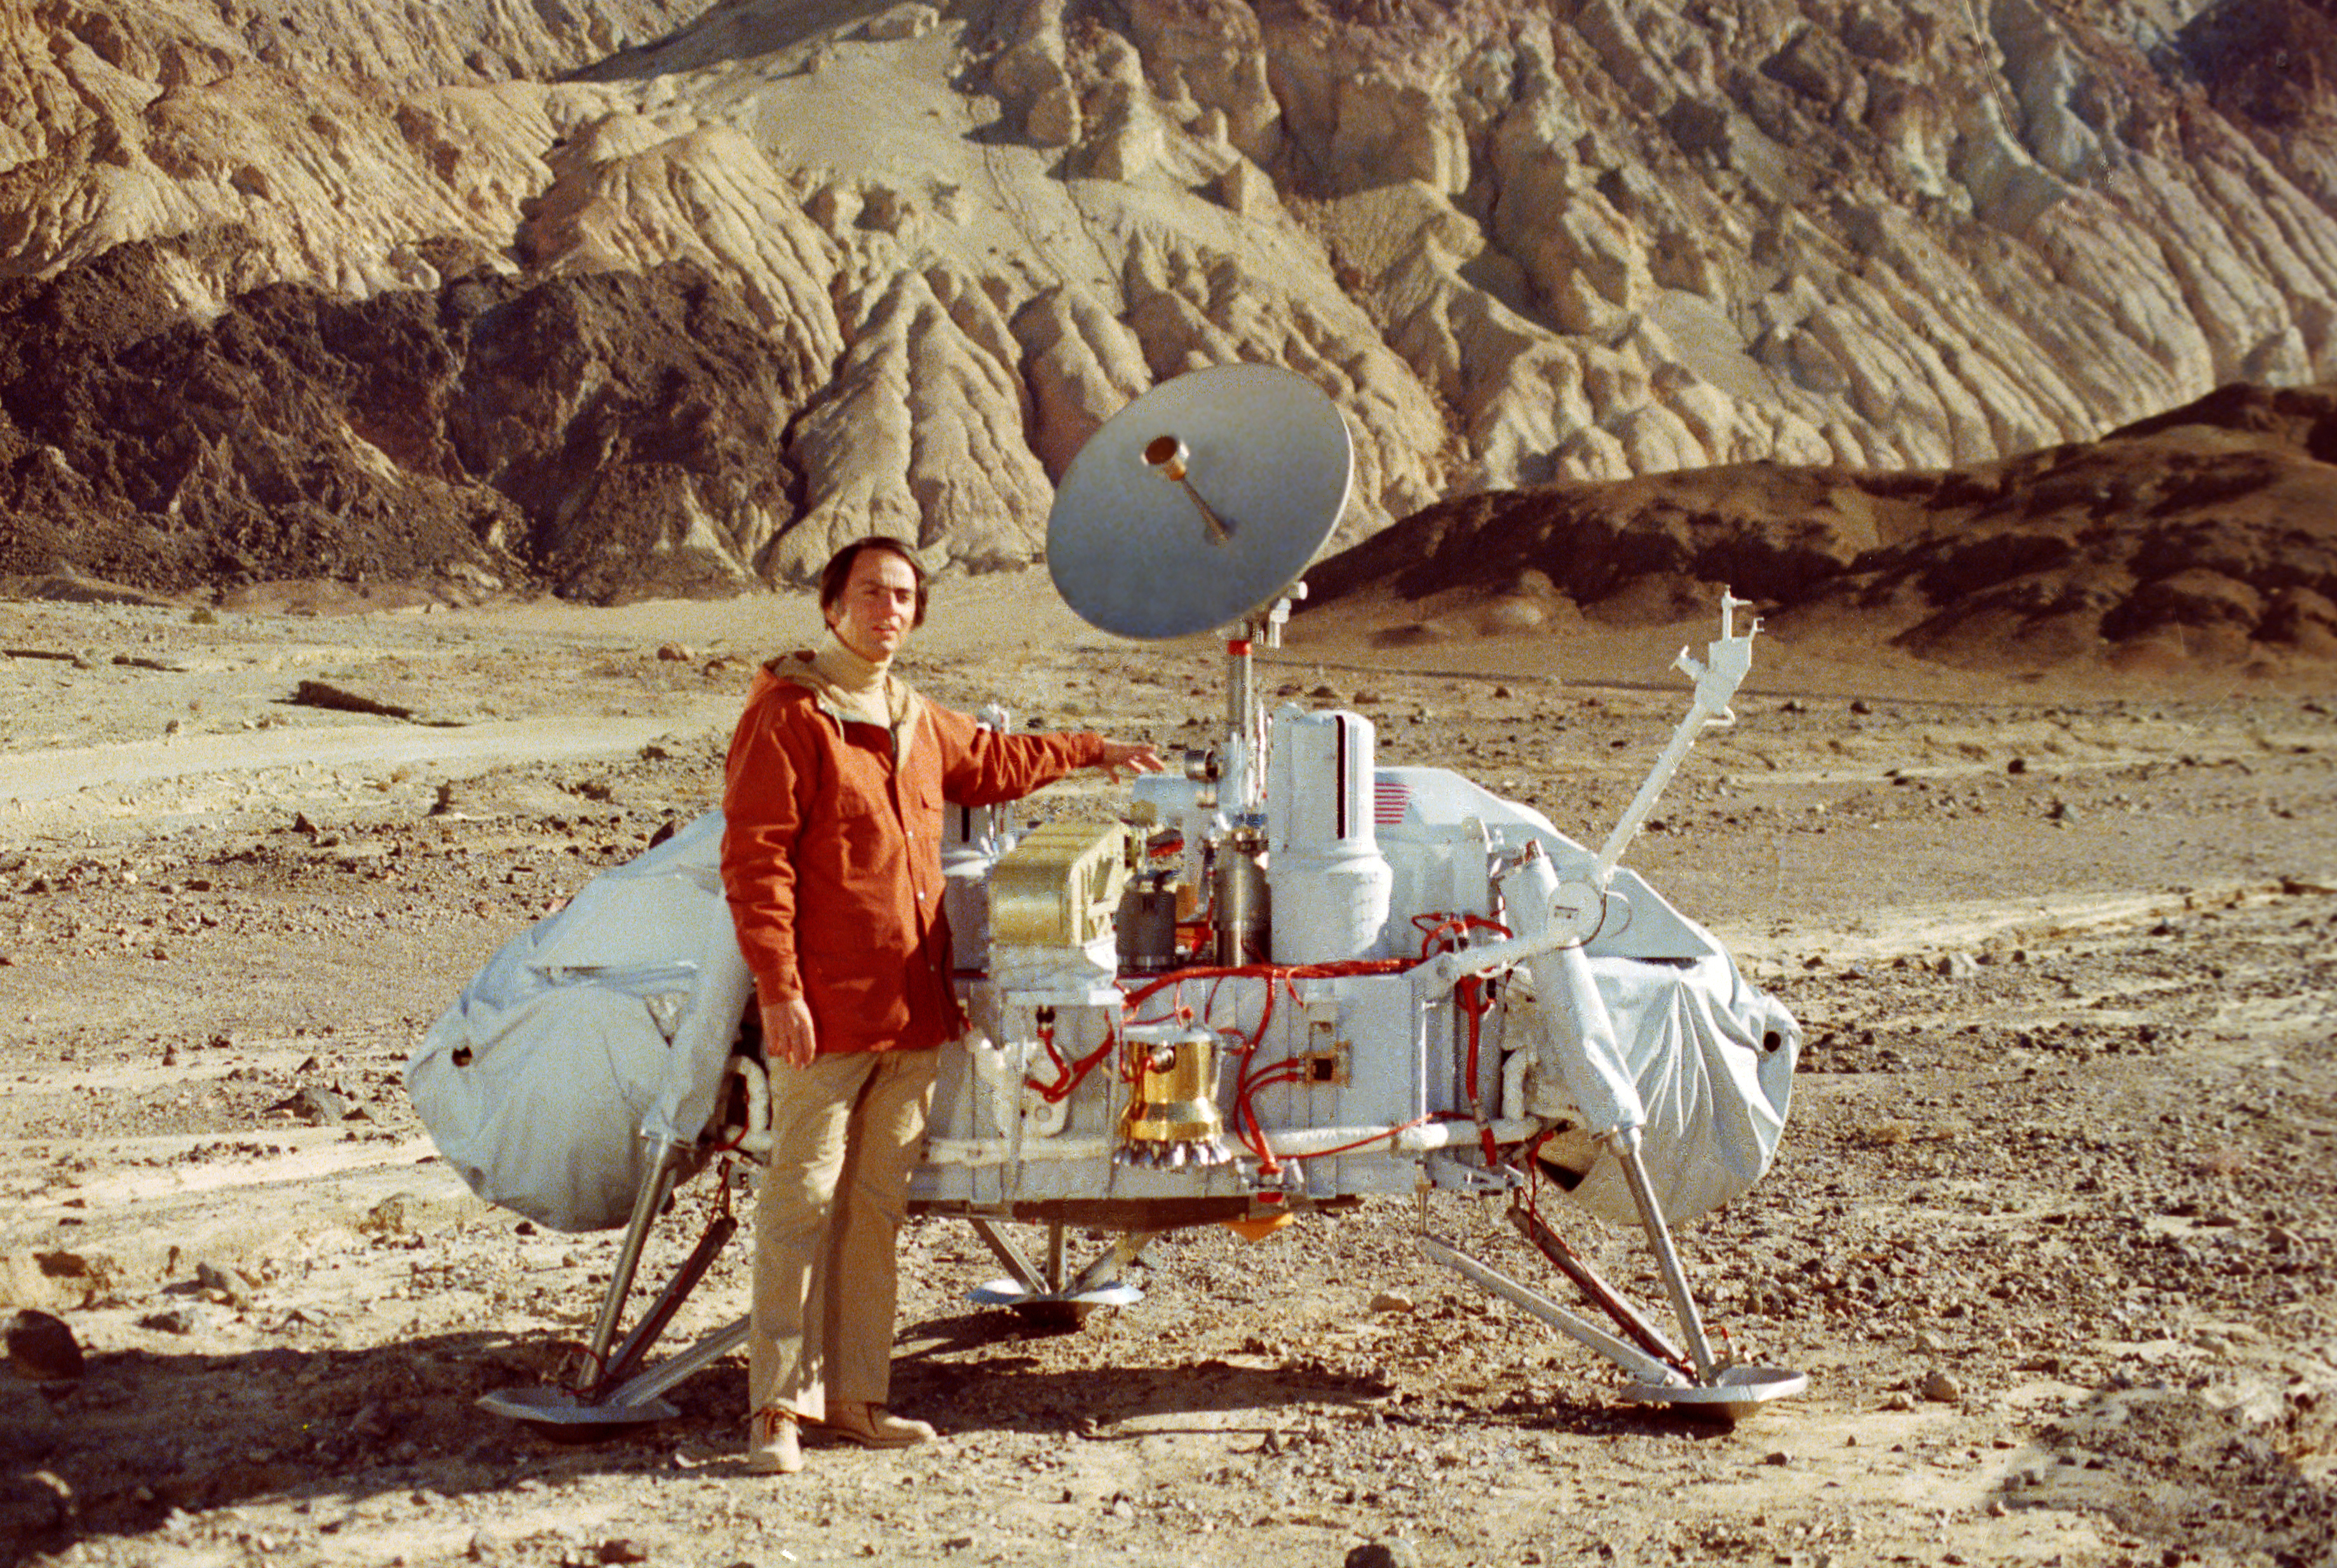
\includegraphics[width=0.4\textwidth]{viking1.jpg}}
	\caption[Los primeros robots espaciales, el Mars 3 y el Viking I]{Imágenes de los primeros robots espaciales: una copia del Mars 3 (a) expuesto en el Museo Memorial de la Cosmonáutica en Moscú, y en Dr. Carl Sagan posando junto a un modelo del Viking I (b) en el Valle de la Muerte, California} \label{fig:vikingmars}
\end{figure}

Desde entonces la robótica ha experimentado en multitud de aplicaciones y formatos con modelos sumamente ambiciosos, como es el caso del IT, diseñado para expresar emociones, el COG, también conocido como el robot de cuatro sentidos, el famoso Sojourner o el Lunar Rover, vehículos con control remoto, y otros mucho mas específicos como el Cypher, un helicóptero robot de uso militar, el guardia de trafico japonés Anzen Taro o los robots mascotas de Sony. En el campo de los robots antropomorfos (androides) se debe mencionar el P3 de Honda que mide 1.60m, pesa 130 Kg y es capaz de subir y bajar escaleras, abrir puertas, pulsar interruptores y empujar vehículos, así como el robot ASIMO de la misma compañía, capaz de desplazarse de forma bípeda e interactuar con las personas.

En general la historia de la robótica la podemos clasificar en cinco generaciones (división hecha por Michael Cancel, director del Centro de Aplicaciones Robóticas de Science Application Inc. en 1984): 
\begin{enumerate}[1.ª Generación]
	\item[1.ª Generación] Robots manipuladores. Son sistemas mecánicos multifuncionales con un sencillo sistema de control, bien manual, de secuencia fija o de secuencia variable.
	\item[2.ª Generación] Robots de aprendizaje. Repiten una secuencia de movimientos que ha sido ejecutada previamente por un operador humano. El modo de hacerlo es a través de un dispositivo mecánico. El operador realiza los movimientos requeridos mientras el robot le sigue y los memoriza.
	\item[3.ª Generación] Robots con control sensorizado. El controlador es una computadora que ejecuta las órdenes de un programa y las envía al manipulador para que realice los movimientos necesarios.
	\item[4.ª Generación] Robots inteligentes. Son similares a los anteriores, pero además poseen sensores que envían información a la computadora de control sobre el estado del proceso. Esto permite una toma inteligente de decisiones y el control del proceso en tiempo real.
\end{enumerate}

Las dos primeras, ya fueron alcanzadas en los ochenta. La tercera generación, que incluye visión artificial, ha avanzado mucho en los ochenta y noventa. La cuarta contempla movilidad avanzada en exteriores e interiores. Y podríamos hablar incluso de una quinta, en la cual entrarían los más modernos sistemas de aprendizaje autónomo y la inteligencia artificial.

El campo de la robótica está en constante expansión, y su popularidad aumenta rápidamente. Ya no solo vemos grandes avances en los robots industriales, como en cadenas de producción, envasado de alimentos o gestión de almacenes, sino que los robots domésticos están cobrando cada vez más importancia. El éxito de los robots aspiradora como Roomba de iRobot\footnote{\url{http://www.irobot.es/}}, la incorporación de aparcamiento automático en coches de todas las gamas o incluso asistentes de conducción autónoma como el autopiloto de Tesla\footnote{\url{https://www.tesla.com/es_ES/}} o prototipos de Google o Apple, los diversos modelos de robots desactivadores de explosivos de los cuerpos de seguridad del mundo, el sistema quirúrgico Da Vinci que permite incluso operar siendo teleoperado desde otro país, los grupos de robots coordinados usados en construcción o misiones de búsqueda y rescate, termostatos inteligentes como el Nest\footnote{\url{https://nest.com/thermostat/meet-nest-thermostat/}} de Google, o la inmensa variedad de drones del mercado ponen de manifiesto que ésta es una tendencia en auge a nivel global.

\begin{figure}[h]
	\centering\includegraphics[width=0.5\textwidth]{esquemarobot.png}
	\caption{Esquema básico del funcionamiento de un robot.}
	\label{fig:esquemarobot}
\end{figure}

Viendo el esquema común a cualquier robot (\textit{Figura \ref{fig:esquemarobot}}), uno de los factores que permiten diseñar, construir y comercializar los robots asegurando una inteligencia y robustez ante situaciones reales es la programación que hay detrás de estos, su software. Usualmente este software tiene varias capas (drivers, middleware y aplicaciones) y presenta unos requisitos específicos dependiendo de las funciones del robot, de su hardware. En los últimos años se han logrado añadir en la fabricación de estos robots ordenadores personales o microprocesadores, principalmente de bajo coste, y sistemas operativos generalistas, lo que permite aumentar la complejidad de sus tareas y el uso de herramientas estándar de desarrollo. Es también el área de la robótica con mayores expectativas de crecimiento e innovación, y donde más importante es la formación para lograr objetivos cada vez más complejos.


\section{Educación en robótica}
\label{sec:intr_educacionrobotica}

El sector de la robótica es un mercado al alza, que demanda científicos e ingenieros de robótica y visión artificial, pero dado que es un campo transversal los profesionales de este sector deben poseer sólidos conocimientos de programación, procesado de imágenes, calculo, álgebra lineal, métodos numéricos, electrónica y electricidad, etc. Esto hace que se puedan realizar aproximaciones desde diferentes puntos de vista. Uno de ellos, más tradicional, es desde las ingenierías eléctricas y electrónicas. La enseñanza desde estas áreas se centra en la construcción del robot, sus partes móviles y mecánicas, sus sensores, motores, su diseño electrónico, procesadores, etc. Otro acercamiento se realiza desde la Informática, poniendo más énfasis en la programación, dado que la inteligencia del robot una vez construido reside en su software.

Cuando los estudiantes de cualquier nivel  educativo construyen un robot están inmersos en un mundo multidisciplinar, dónde la geometría, la trigonometría, la electrónica, la programación, el  control, la mecánica, etc, proporcionan las capacidades básicas que redundarán en el éxito de dicha tarea integradora. Aparte de los conceptos que le son propios, la robótica genera entornos propicios para la colaboración, y el trabajo en equipo donde los niños y jóvenes tienen la oportunidad de aprender y practicar las habilidades  denominadas como las 4C del siglo XXI\footnote{Según la Asociación para las habilidades del siglo XXI (\textit{Partnership for 21st Century Skills}] \url{http://www.p21.org/}}:
\begin{itemize}
	\item Pensamiento Crítico: habilidad imprescindible para un buen aprendizaje. Se basa en la razón efectiva, utilizando varios tipos de razonamiento y analizando la interacción de las partes de un todo, en el análisis y evaluación de las pruebas, argumentos y puntos de vista, en la interpretación de la información y extracción de conclusiones, y en la resolución de problemas.
	\item Comunicación: se basa principalmente en la articulación de pensamientos e ideas en diferentes vías, en la escucha eficaz y en el uso de múltiples medios y tecnologías.
	\item Colaboración: Se basa en la capacidad para trabajar de manera eficaz y respetuosa en diversos equipos, en la voluntad de compromiso en la consecución de objetivos comunes y en la asunción de responsabilidades, tanto compartidas como individuales.
	\item Creatividad: se basa en el pensamiento creativo, usando técnicas de generación de ideas y elaborando, perfeccionando, analizando y evaluando ideas originales, Y en el trabajo creativo, desarrollando y comunicando nuevas ideas de manera efectiva, siendo abierto y receptivo a nuevas ideas y perspectivas o contribuyendo con ideas creativas en el campo de trabajo.
\end{itemize}

Actualmente en nuestro país, la robótica aparece en los cursos de secundaria y de formación profesional, aunque se realiza fundamentalmente en la universidad con algunos títulos de grado y postgrado específicos. 

La formación en robótica, en términos generales, sólo suele aparecer con suficiente contenido en los programas de formación profesional en las asignaturas técnicas  de  las  ramas correspondientes. En  concreto, aparece en el título de Grado Medio de Técnico en Mecanizado (lenguajes de programación de robots), y en una parte del módulo de Sistemas de Control Secuencial en ciclo formativo de Grado Superior del titulo de Técnico Superior en Sistemas de Regulación y Control Automáticos.

En la enseñanza secundaria la robótica permite acercar la tecnología a los niños y motivarles para aprender conceptos básicos de ciencias, tecnología, ingeniería y matemáticas. Estas áreas han visto reducido el número de estudiantes en los últimos años, y numerosos gobiernos han realizado grandes inversiones para incentivar a los estudiantes a orientar sus estudios hacia estos campos. En la Comunidad de Madrid se ha introducido\footnote{Decreto 48/2015} la asignatura \textit{Tecnología, programación y robótica} en el curriculum oficial de la ESO (Educación Secundaria Obligatoria). 

Fuera de esta asignatura específica aparece, generalmente asociado a contenidos de automatismos, tan solo en un par de temas de algunas de las pocas asignaturas de tecnología: Tecnología Industrial 3, obligatoria en 3º, y Tecnología Industrial 4, optativa de 4º curso. En bachillerato, en la modalidad Tecnología, los contenidos de robótica suelen aparecer marginalmente en las asignaturas de Tecnología 1 y 2, del Bachillerato de la Modalidad Tecnología. Generalizando, se puede decir que la mayoría del alumnado no adquiere una formación específica importante en robótica tras su paso por la Enseñanza Secundaria. 

En esta etapa se utilizan plataformas como los diferentes robots de LEGO\footnote{Lego posee toda una gama pensada para la educación: \url{https://education.lego.com/}} (Mindstorms, NXT, Evo, WeDo, RCX) o placas con procesadores Arduino\footnote{\url{https://www.arduino.cc/}} a las que se conectan diversos sensores, actuadores, servos, etc. Con estas plataformas se introducen las bases de la programación con lenguajes sencillos, usando entornos de prácticas donde completar código ya estructurado o entornos gráficos para niños como Scratch, RCX-code, mbot Blockly. Cabe mencionar el curso de JdeRobot-Kids\footnote{\url{http://jderobot.org/JdeRobot-kids}}, que utiliza Arduino como placa programable, mBot como robot móvil y Python como lenguaje para introducir conceptos básicos de tecnología a alumnos jóvenes e iniciarles en robótica y programación, haciéndolo de manera atractiva y enseñando conceptos interesantes de mecánica, electrónica e informática. El carácter del curso es práctico, de \textit{aprender haciendo}.

En la enseñanza superior o universitaria, tradicionalmente se imparten asignaturas de robótica en las escuelas de ingeniería, ya sea industrial, electrónica, informática, etc. La enseñanza de la robótica y materias afines como la visión por computador,la inteligencia artificial y el aprendizaje automático, de interés para nuestra comunidad, encuentra cobijo en las actuales enseñanzas de Grado, principalmente en el ámbito industrial, aunque también en el ámbito informático. 

En España existen grados y varios másteres con contenidos en robótica. Una de las titulaciones de Grado en el ámbito industrial que presentan estos contenidos es el Grado en Ingeniería Electrónica y Automática de la Universidad de Zaragoza, que oferta al estudiante, dentro de la tecnología específica de Electrónica Industrial, algunas asignaturas que como Ingeniería de Control, Robótica Industrial o Automatización Industrial, todas relacionadas con la robótica. Adicionalmente esta titulación oferta un  módulo optativo de 30 ECTS denominado “Automatización y Robótica”. La titulación de Grado en Ingeniería en Informática de la Universidad de Málaga oferta al estudiante la asignatura \textquotedblleft Robótica\textquotedblright  de 6 créditos ECTS. En el Grado en Ingeniería Informática de la Universidad de Zaragoza se pueden encontrar las asignaturas “Inteligencia Artificial” y “Aprendizaje”, de 6 créditos cada una. 

Dentro de los títulos de Máster muchas universidades incluyen más asignaturas de robótica, dado que son estudios más especializados y pueden dedicar una mayor carga lectiva a estos temas. Por ejemplo, el Máster en Ingeniería Informática de la Universidad Carlos III de Madrid presenta entre sus asignaturas “Sistemas de producción automatizados” y “Diseño de Sistemas Inteligentes”, de 3 y 6 créditos ECTS respectivamente. Aunque también existen Másteres totalmente dedicados a este ámbito, como por ejemplo el Máster Universitario en Robótica y Automatización,  también de la Universidad Carlos III de Madrid.

Los estudios oficiales de Máster Erasmus Mundus integran un conjunto de cursos de alto nivel que son impartidos por un consorcio formado, por al menos, tres universidades de tres países europeos diferentes. Son cursos integrados porque tienen un plan de estudios conjunto y comportan un período de estudio en al menos dos de las universidades participantes. Este tipo de másteres están pensados para fortalecer la cooperación europea y los vínculos internacionales en la enseñanza superior, y presentan estudios especializados en este sector, como el Erasmus Mundus Masters in VIsion and robotics (Universidad de Gerona, Université de Bourgogne y Heriot-Watt University). El Máster VIBOT se estructura en cuatro semestres que proporcionan una formación integral en los ámbitos de la Visión por Computador y la Robótica.

En Estados Unidos, las universidades más punteras en tecnología, como Stanford o el MIT, cuentan con programas de grado y postgrado entre sus planes de estudios.

Las asignaturas de robótica impartidas en la universidad tienen un enfoque práctico, de forma que la interacción del alumno con los robots facilita el aprendizaje y entendimiento de los conceptos teóricos mediante un aprendizaje activo. Es habitual el uso de plataformas específicas para la programación del robot como ROS (sección \ref{sec:inf_ros}) o MATLAB\footnote{\url{https://es.mathworks.com/products/matlab.html}} y su paquete Simulink\footnote{\url{https://es.mathworks.com/products/simulink.html}}. Otros se centran en el diseño y modelado del robot.

\section{Entorno docente JdeRobot-Academy }
\label{sec:intr_entornodocente}

Desde la Universidad Rey Juan Carlos se plantea un entorno de enseñanza universitaria llamado \textit{JdeRobot-Academy}, dentro de la plataforma JdeRobot (\textit{Sección \ref{sec:inf_jderobot}}). Orientado para realizar cursos universitarios de 12-14 semanas, plantea ocultar todo el middleware al alumno y dejar que se centre en la programación de los algoritmos. De esta manera el alumno desarrolla software para una tarea determinada sin necesidad de desarrollar el software que conecta los elementos del robot, por lo que es perfecto para cursos de introducción a la robótica o que hagan énfasis en la programación de robots ya construidos. En la Universidad Rey Juan Carlos se ha utilizado en la asignatura \textquotedblleft Robótica\textquotedblright, en el grado en Ingeniería Telemática, en la asignatura \textquotedblleft Visión en Robótica\textquotedblright, en el Máster de Visión Artificial, y en varios cursos de introducción a la robótica y a los drones, así como en el campeonato PROGRAMAROBOT\footnote{\url{http://jderobot.org/Campeonato-programacion-de-robots}}.

Este entorno docente está compuesto de diferentes prácticas independientes que siguen el mismo planteamiento: se propone un problema robótico y el estudiante programa la inteligencia del robot para resolverlo. Se pueden diferenciar una serie de capas que componen dichas practicas. La capa más baja es donde se encuentra el robot, simulado o real, con todos los sensores o actuadores que lo componen. En la siguiente capa se encuentran los drivers del robot, que permiten acceder a los sensores y actuadores del robot. Y en la última capa se encuentra la aplicación, que analiza los datos de los sensores y da órdenes a los actuadores. En esta capa se encuentra el código de toma de decisiones y planificación. Aquí se encuentra una parte de código específico y necesario para el funcionamiento del robot y otra parte en blanco que el alumno debe completar para resolver con éxito el problema planteado. 

Dichas prácticas pueden realizarse sobre robots reales o simulados, aunque generalmente es conveniente comenzar con la simulación antes de pasar a escenarios reales. Se apoyan, por tanto, en el simulador Gazebo (\textit{Sección \ref{sec:inf_gazebo}}), y usan lenguajes de programación como Python o C++. Aunque el principal sistema operativo para utilizar esta plataforma es Linux, ya sea Ubuntu o Debian, se ha usado la interfaz web de Gazebo para poder lanzarlo cómodamente en Windows y MacOS. Esto se ha conseguido lanzando el servidor de Gazebo y los drivers en un contenedor Docker, el cual permite ejecutar la aplicación de forma nativa en cada sistema operativo y conectarse mediante una aplicación web al simulador Gazebo para ver el mundo de la simulación.

Algunas de las prácticas desarrolladas son:
\begin{itemize}
	\item \textit{Drones: persecución}. En esta práctica el alumno programa un drone \textit{gato} que persigue a otro drone \textit{ratón} (\textit{Figura \ref{fig:gatoraton}}). El mundo de Gazebo no presenta obstáculos para facilitar la programación del robot, y los drones son similares a los AR.Drone de Parrot\footnote{\url{https://www.parrot.com/es/drones/parrot-ardrone-20-elite-edition}} . Hay varios niveles de \textit{ratón} disponibles, cuya dificultad de persecución va en aumento. El drone \textit{gato} posee una cámara frontal, una cámara cenital, inclinómetros y GPS, y facilita una interfaz de control que acepta órdenes simples como avance hacia delante, lateral, ascenso, etc. El objetivo del estudiante es programar los elementos de percepción visual necesarios para que el drone \textit{gato} localice al drone \textit{ratón} y los movimientos necesarios para la persecución del drone \textit{ratón}. También se incluye un componente de evaluación automática y objetiva, el cual puntúa el número de segundos que la distancia con el drone \textit{ratón} está por debajo de un umbral.
	
	Esta practica sirve para enseñar elementos de control y percepción visual, necesarios para buscar y encontrar al otro drone y para reaccionar en base a sus movimientos., para lo cual son necesarios conocimientos en procesamiento de imágenes y nociones de manejo de OpenCV\footnote{\url{http://opencv.org/}}. También se enseñan nociones como el controlador PID, consistente en un mecanismo de control basado en un algoritmo que, por ejemplo, permite controlar el rumbo del drone frente a cambios de dirección del drone perseguido, y elementos de control basado en casos, por ejemplo, un caso podría ser buscar al robot ya que no aparece en los sensores, y otro modificar la dirección cuando el drone perseguido se acerca a los bordes de la imagen captada por la cámara.

\begin{figure}[h]
	\centering\includegraphics[width=0.7\textwidth]{gatoraton.png}
	\caption{Robot ArDrone en Gazebo persiguiendo a otro ArDrone dentro de una práctica.}
	\label{fig:gatoraton}
\end{figure}
	
	\item \textit{Control visual: sigue líneas}. En esta práctica el alumno debe conseguir que un robot Kobuki (\textit{Figura \ref{fig:kobuki}}) siga la línea roja de un circuito en el menor tiempo posible. El estudiante debe realizar los filtros de percepción necesarios para que el robot siga la línea roja y los movimientos del robot para mantenerse en la trayectoria adecuada.
	
	Esta práctica sirve para enseñar técnicas de percepción visual, de control reactivo, control basado en casos y de controladores PID.

\begin{figure}[h]
	\centering\includegraphics[width=0.4\textwidth]{turtlebot_simulado.png}
	\caption{Robot kobuki en Gazebo.}
	\label{fig:kobuki}
\end{figure}
	
	\item \textit{Fórmula 1: nacegación local}. En esta práctica el alumno debe programar un coche de Fórmula 1 (\textit{Figura \ref{fig:f1}}) para que complete una vuelta a un circuito de carreras esquivando los obstáculos que se encuentre en el camino. El robot cuenta con sensores de odometría, GPS y un sensor láser, y la interfaz de movimiento admite órdenes simples como velocidad de avanze o de giro.
	
	Para el desarrollo de esta practica se abordan algoritmos de navegación local como
	VFF (virtual force field) o campos virtuales, además de técnicas de percepción visual, de control reactivo o controladores PID.
	
\begin{figure}[h]
	\centering\includegraphics[width=0.4\textwidth]{f1.png}
	\caption{Robot de Fórmula 1 en un circuito en Gazebo.}
	\label{fig:f1}
\end{figure}
	
	\item \textit{TeleTaxi: navegación global}. En esta práctica el alumno debe conseguir que un coche vaya de un punto a otro cualquiera de una ciudad (\textit{Figura \ref{fig:teletaxi}}). El coche, taxi, tiene un sensor GPS y una interfaz como la del Fórmula 1. El alumno debe programar un algoritmo de navegación para que alcance la posición objetivo en un mapa conocido.
	
	En esta práctica se abordan, además de los elementos de control reactivo, algoritmos de planificación de caminos como Gradient Path Planning. En esta práctica no se necesitan elementos de percepción visual, ya que el taxi se guiará usando el GPS.

\begin{figure}[h]
	\centering\includegraphics[width=0.6\textwidth]{teletaxi-city2.png}
	\caption{Robot taxi en una ciudad en Gazebo.}
	\label{fig:teletaxi}
\end{figure}
	
	\item \textit{Visión: reconstrucción 3D}. En esta práctica el alumno debe conseguir que un robot Pioneer (\textit{Figura \ref{fig:mundo3D}}) reproduzca en 3D los elementos que se le presentan. Este robot está equipado con un par estéreo de cámaras. Para conseguir su objetivo, el alumno debe programar un algoritmo de reconstrucción 3D clásico de tres pasos: detección de puntos de interés en las dos imágenes, emparejamiento de píxeles homólogos entre ambas, y triangulación espacial para calcular el punto tridimensional que origina cada pareja de píxeles homólogos.
	
	En esta práctica no se necesita que el robot se mueva, pero sí tiene una alta carga visual, pro lo que se abordarán técnicas de procesado de imagen y de percepción visual.
	
\begin{figure}[h]
	\centering\includegraphics[width=0.5\textwidth]{mundo3D.png}
	\caption{Robot Pioneer en Gazebo frente al conjunto de objetos a escanear.}
	\label{fig:mundo3D}
\end{figure}

\end{itemize}

Nuestro objetivo con este trabajo es aumentar las posibilidades de esta plataforma, creando nuevos escenarios que aporten valor y funcionalidades nuevas a las prácticas ya existentes o desarrollando nuevas herramientas que permitan añadir prácticas más variadas a la colección.

En los siguientes capítulos cubriremos todos los elementos necesarios para lograr este objetivo. En el segundo capítulo abordaremos los objetivos marcados para este proyecto, así como los requisitos necesarios para cumplirlos y la metodología que usaremos. En el tercer capítulo expondremos los elementos usados como infraestructura, las herramientas que nos permitirán completar nuestra tarea. En el cuarto y quinto capítulo veremos las soluciones a las que hemos llegado para alcanzar los objetivos planteados, y en el sexto las conclusiones obtenidas de la realización de este proyecto, así como los futuros pasos a seguir.












